\documentclass[a4paper]{article}
\usepackage{ifpdf}
\oddsidemargin=-5mm
\evensidemargin=-5mm\marginparwidth=.08in \marginparsep=.01in
\marginparpush=5pt\topmargin=-15mm\headheight=12pt
\headsep=25pt
\footskip=30pt
\textheight=25cm
\textwidth=17cm\columnsep=2mm
\columnseprule=1pt\parindent=15pt\parskip=2pt
\ifpdf
  % one of these two:
  \usepackage[pdftex]{graphicx}  % note the x at the end
  %\usepackage[pdftex]{epsfig}

  % hyperref should be the last package loaded:
  \usepackage[pdftex]{hyperref}
\else
  % one of these two:
  \usepackage[dvips]{graphicx}  % note the x at the end
  %\usepackage[dvips]{epsfig}

  % make the command \href from hyperref available as a 'print only'
  \newcommand{\href}[2]{#2}
\fi


\begin{document}
\begin{center}
\bf Semestralni projekt PAR 2007/2008:\\[5mm]
    Paralelni algoritmus pro reseni problemu UPO\\[5mm] 
       Miloslav Cinibulk\\
       Tomas Horacek\\[2mm]
5. rocnik, obor pocitace, K336 FEL CVUT, Karlovo nam. 13, 121 35 Praha 2\\[2mm]
\today
\end{center}

\section{Definice problemu a popis sekvencniho algoritmu}

\subsection{Vstupni data}
\begin{itemize}
	\item n = prirozene cislo
	\item k = prirozene cislo radu jednotek
	\item G = neorietovany neohodnoceny graf o n uzlech a stupni nejvyse k (zvolte standardni
	      reprezentaci s ocislovanymi uzly 1,...,n, napr. seznam sousedu nebo matici sousednosti).
	      Graf G nemusi byt souvisly.
\end{itemize}
\subsection{Ukol:}
Nalezt minimalni podmnozinu uzlu C, ktera pokryva kazdou hranu, tzn. kazda hrana je incidentni
s aspon s jednim uzlem z C.
\subsection{Vystup algoritmu:}
Vypis prvku mnoziny C (reseni existuje vzdy).
\subsection{Sekvencni algoritmus:}
Sekvencni algoritmus je BB-DFS s omezenou hloubkou prohledavaneho prostoru. Stav je dan obsahem
mnoziny C. Stav je pripustny, je-li C pokryti. Cena, kterou minimalizujeme, je $|$C$|$.
Pokryti C lze budovat bud pridavanim uzlu pocinaje prazdnou mnozinou, kdy se provadi navrat,
pokud jsou vsechny hrany pokryty, nebo odebiranim uzlu z nadbytecne velkeho pokryti, kdy se navrat
provadi, pokud nelze zadny uzel odebrat, aniz by se narusilo pokryti.

Dolni mez neni znama.

Trivialni horni mez $|$C$|$ je n/2.

Na zacatku algoritmu je nactena matice incidence grafu. Na zasobnik se vzdy ukladaji tato data:

\begin{itemize}
	\item cislo uzlu s kterym prave pracujeme
	\item to, zda odebirame uzel, nebo ponechavame uzel
	\item pocet zatim vybranych uzlu
	\item bitove pole vybranych uzlu
	\item pole hran s pocty uzlu s kterymi inciduji
\end{itemize}

Pocatecni stav algoritmu je takovy, ze jsou vybrany vsechny uzly. Pak algoritmus postupne zkousi
odebrat ruzne kombinace uzlu, ovsem vzdy tak, aby hrana kazda hrana incidovala alespon
s jednim uzlem (proto zasobnik obsahuje pole poctu uzlu incidujicich s jednotlivymi hranami).

Nejlepsi reseni se ukladaji do globalni promene a po projiti vsech smysluplnych kombinaci
odebrani uzlu se nejlepsi reseni vypise.

\section{Popis paralelniho algoritmu a jeho implementace v MPI}

Paralelni algoritmus je typu PBB-DFS-V. Princip algoritmu je stejny jako u sekvenciho reseni.

Na zacatku proces 0 nacte graf a rozesle ho ostatnim procesum. Prace se mezi procesi
rozesila formou polozky zasobniku. Po rozeslani grafu zacne proces 0 pocitat
a kdyz ma na zasobniku dostatecny pocet polozek pro vsechny procesy,
tak jim rozesle praci.

Behem vypoctu se muze stat, ze nektery proces dopocita svoje reseni. V tom pripade
se zepta sveho souseda, jestli mu nepreda cast prace a takto se pta v kruhu
dal, dokavad nejakou neziska.

Ukonceni paralelniho vypoctu je provedeno peskovymi algoritmem.

\section{Namerene vysledky a vyhodnoceni}

\subsection{Instance}

Instacemi byly 3 ruzne nahodne grafy se 70 uzly, kde 2 uzly maji stupen 30 a ostatni mensi.

\subsection{Namerene vysledky}

\begin{figure}[ht]
\centerline{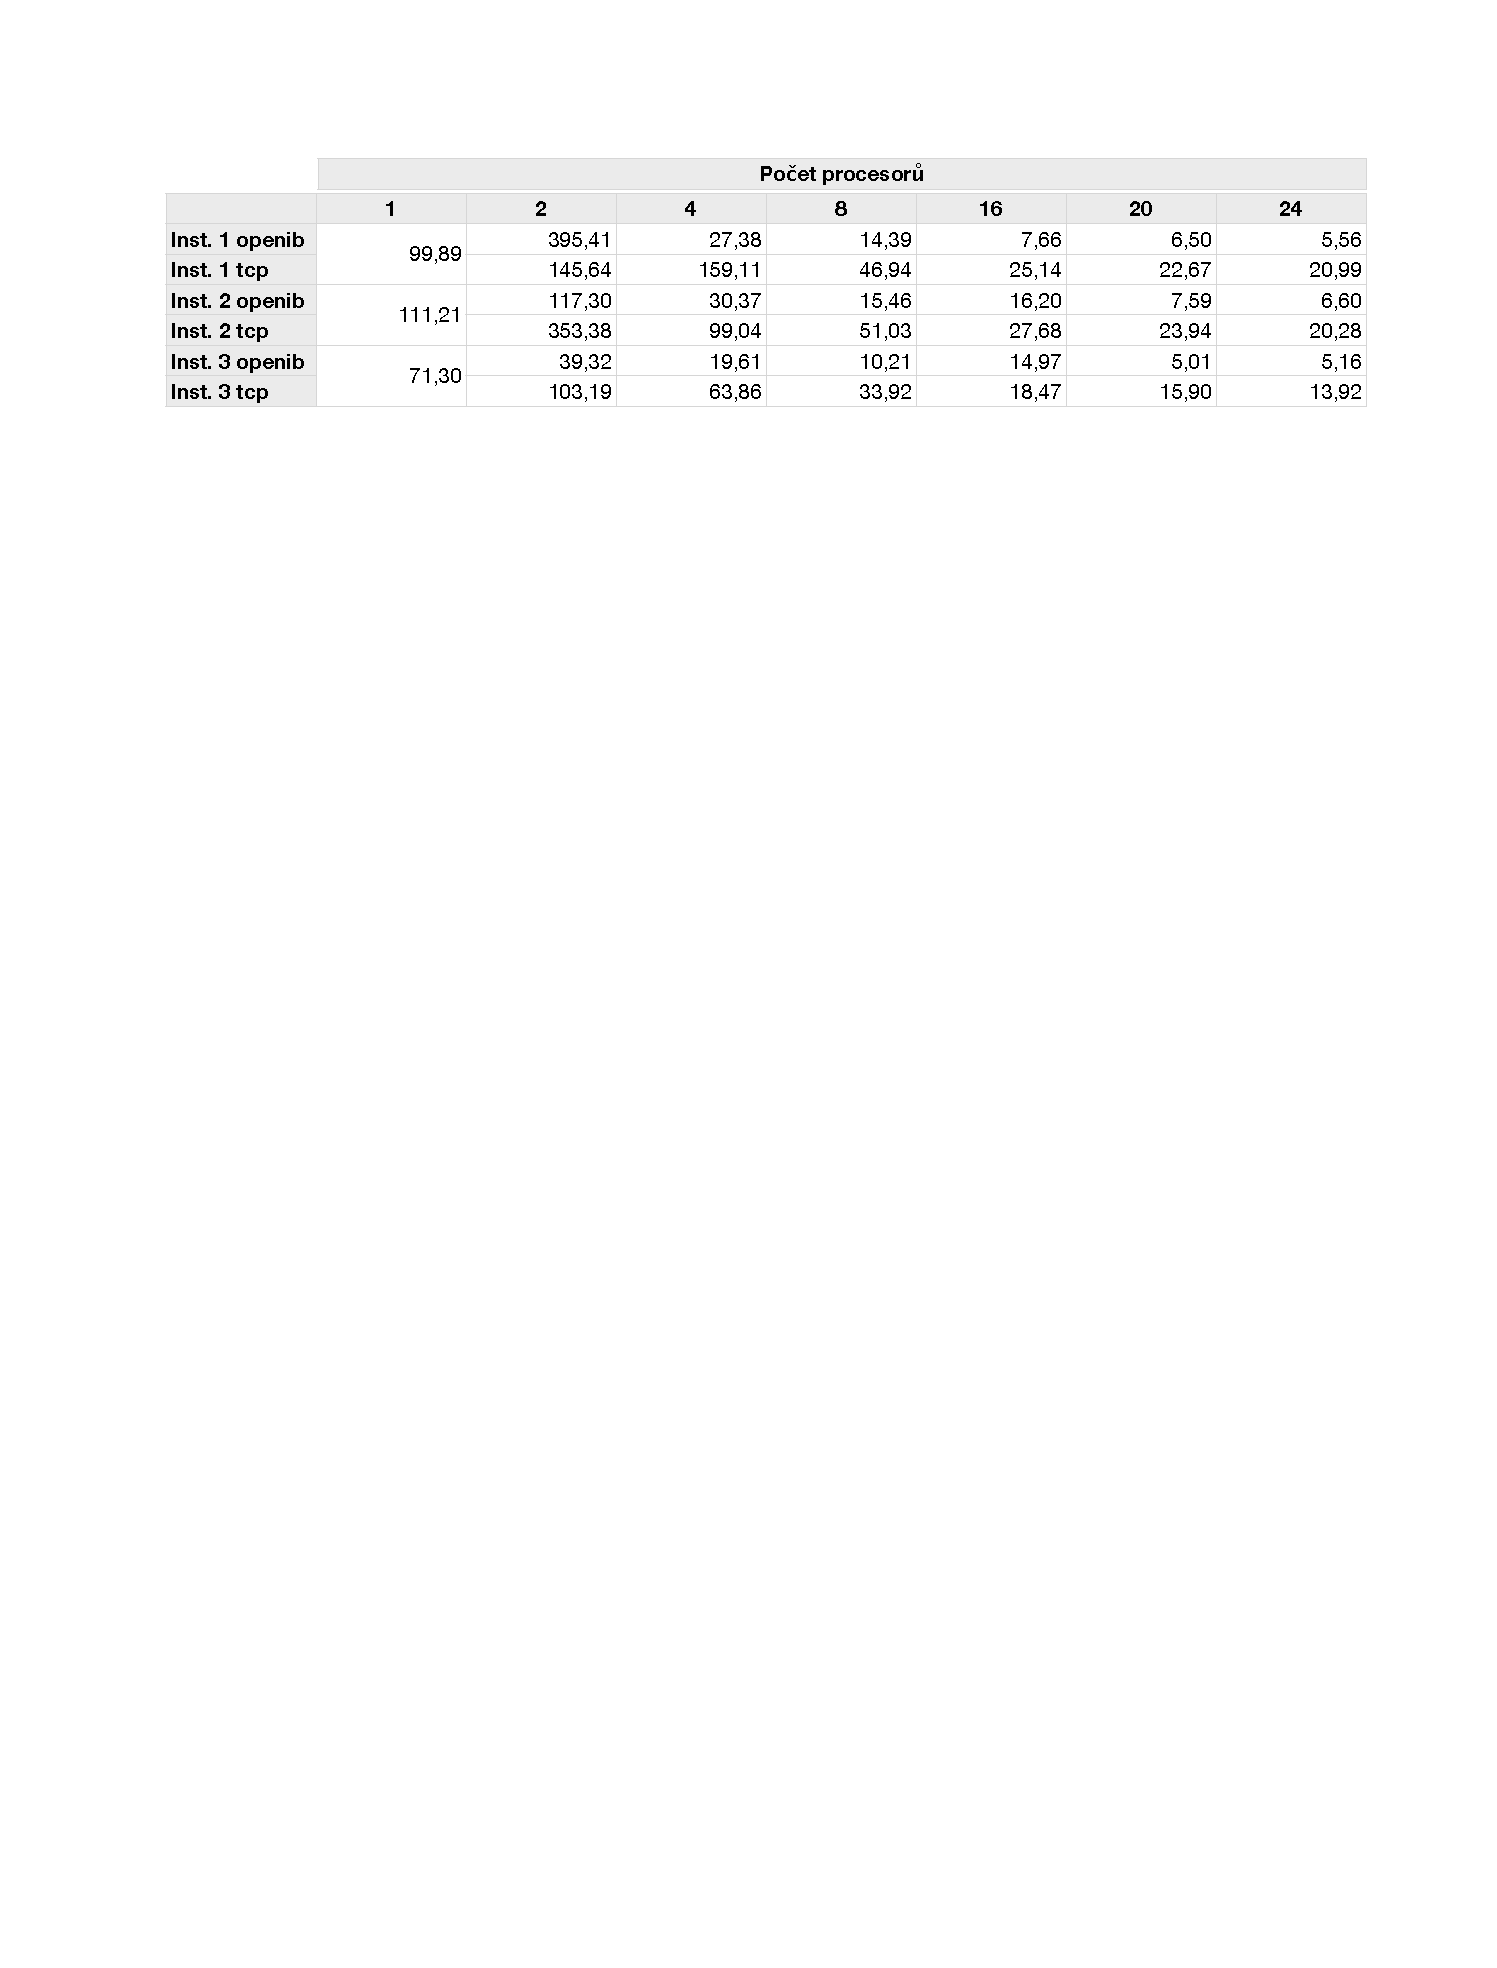
\includegraphics[width=\textwidth]{table-abs.pdf}}
\caption{Namerene vysledky delky vypoctu [s]}
\label{table-abs}
\end{figure}

\begin{figure}[ht]
\centerline{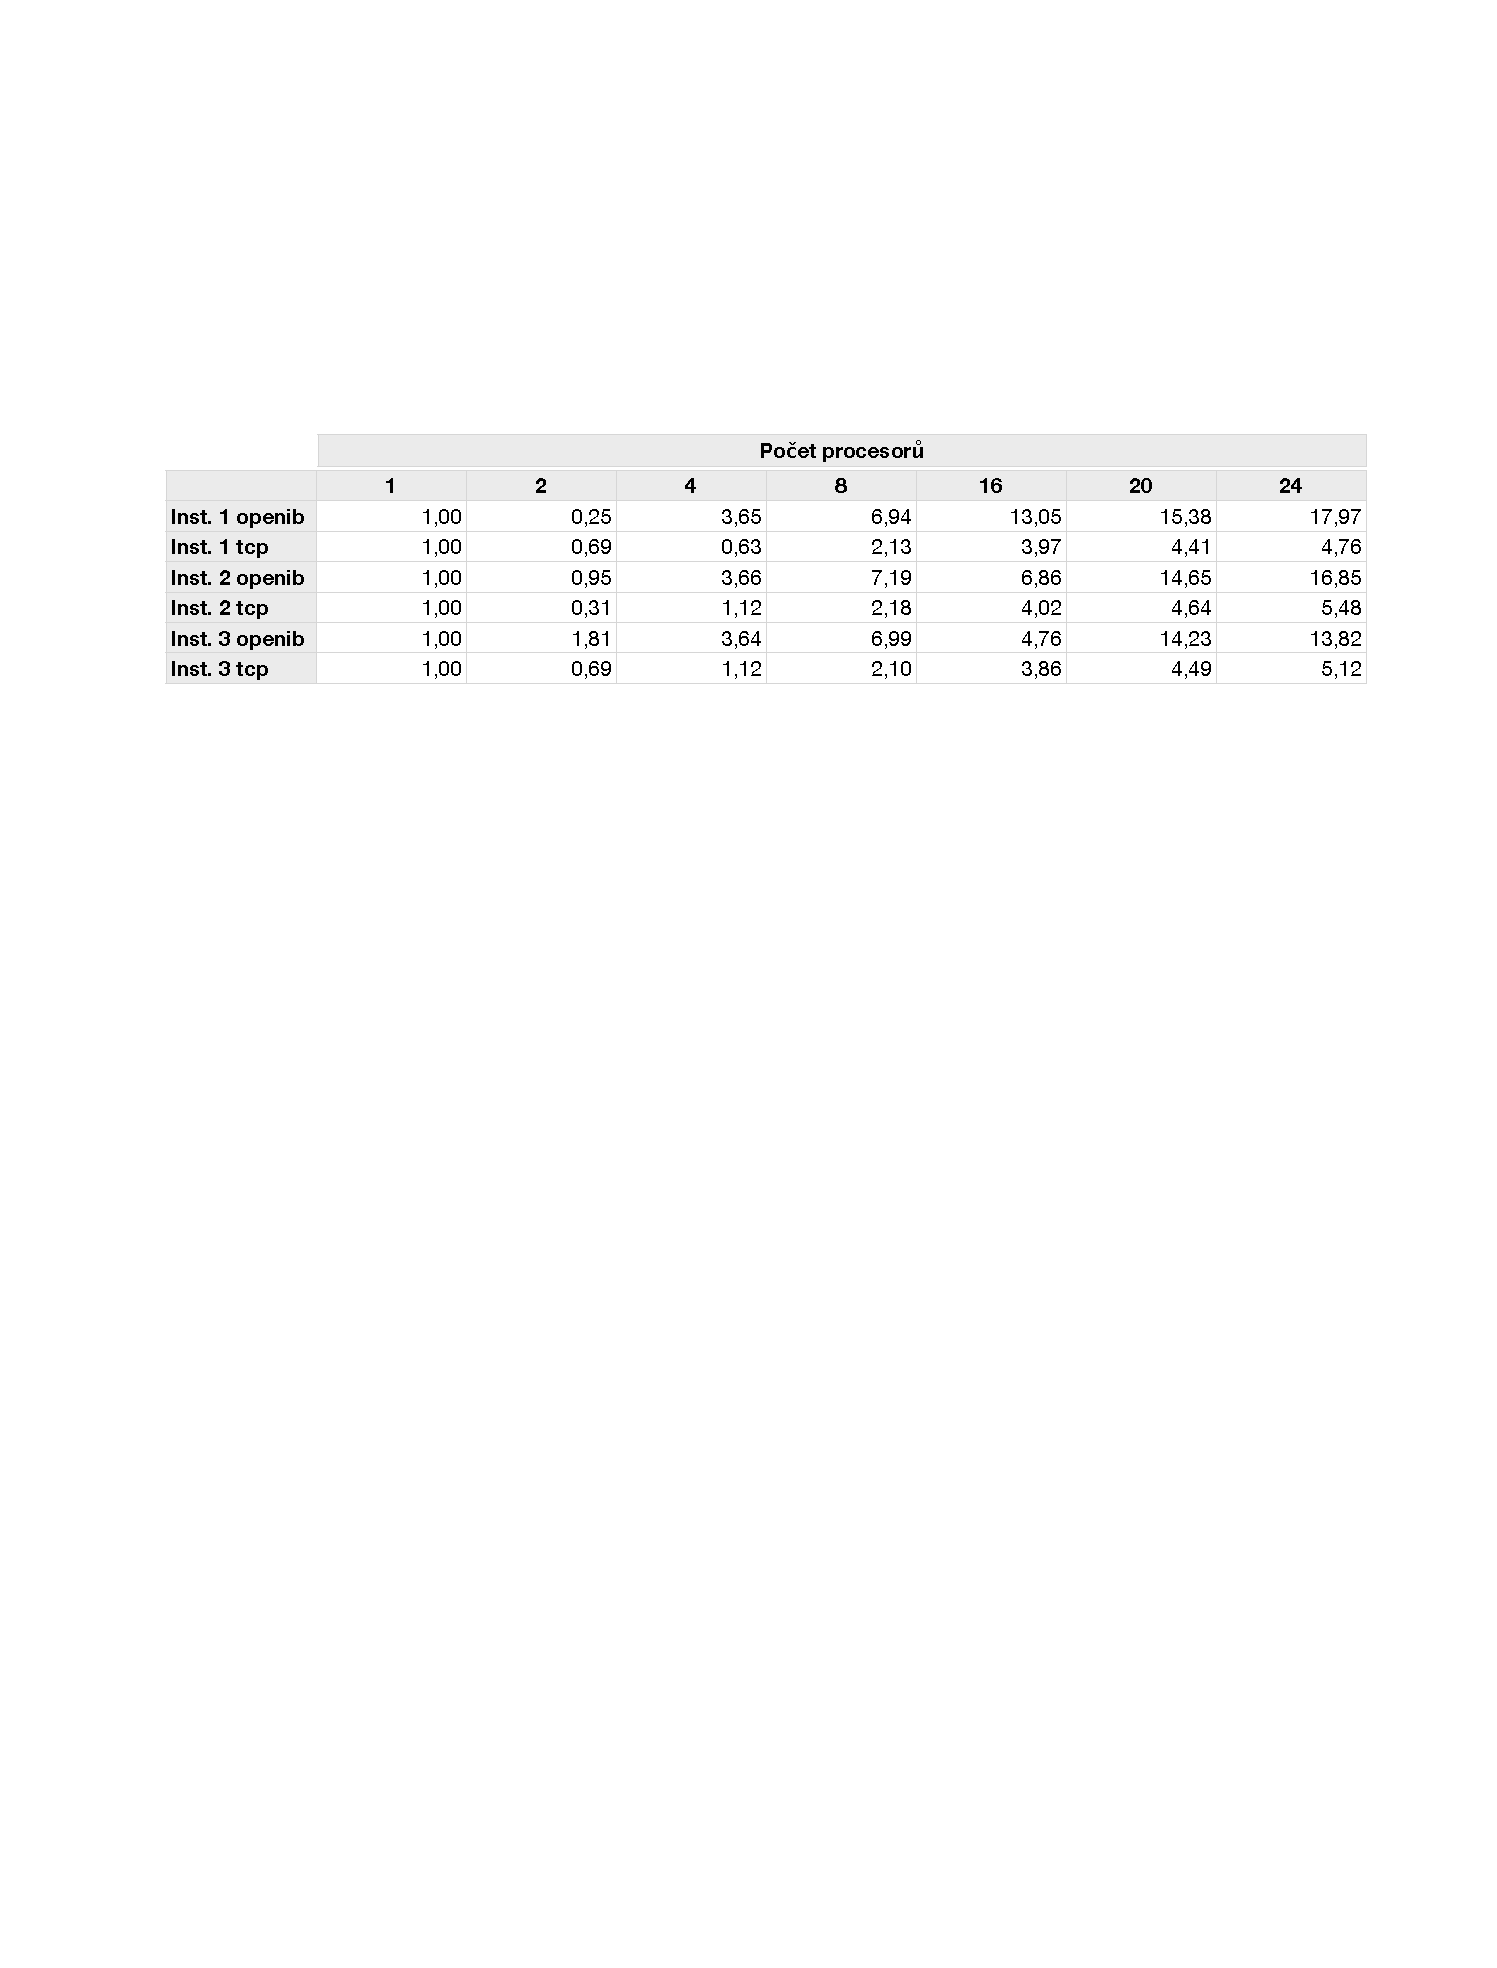
\includegraphics[width=\textwidth]{table-rel.pdf}}
\caption{Relativni zrychleni vypoctu proti sekvencnimu algoritmu}
\label{table-rel}
\end{figure}

\begin{figure}[ht]
\centerline{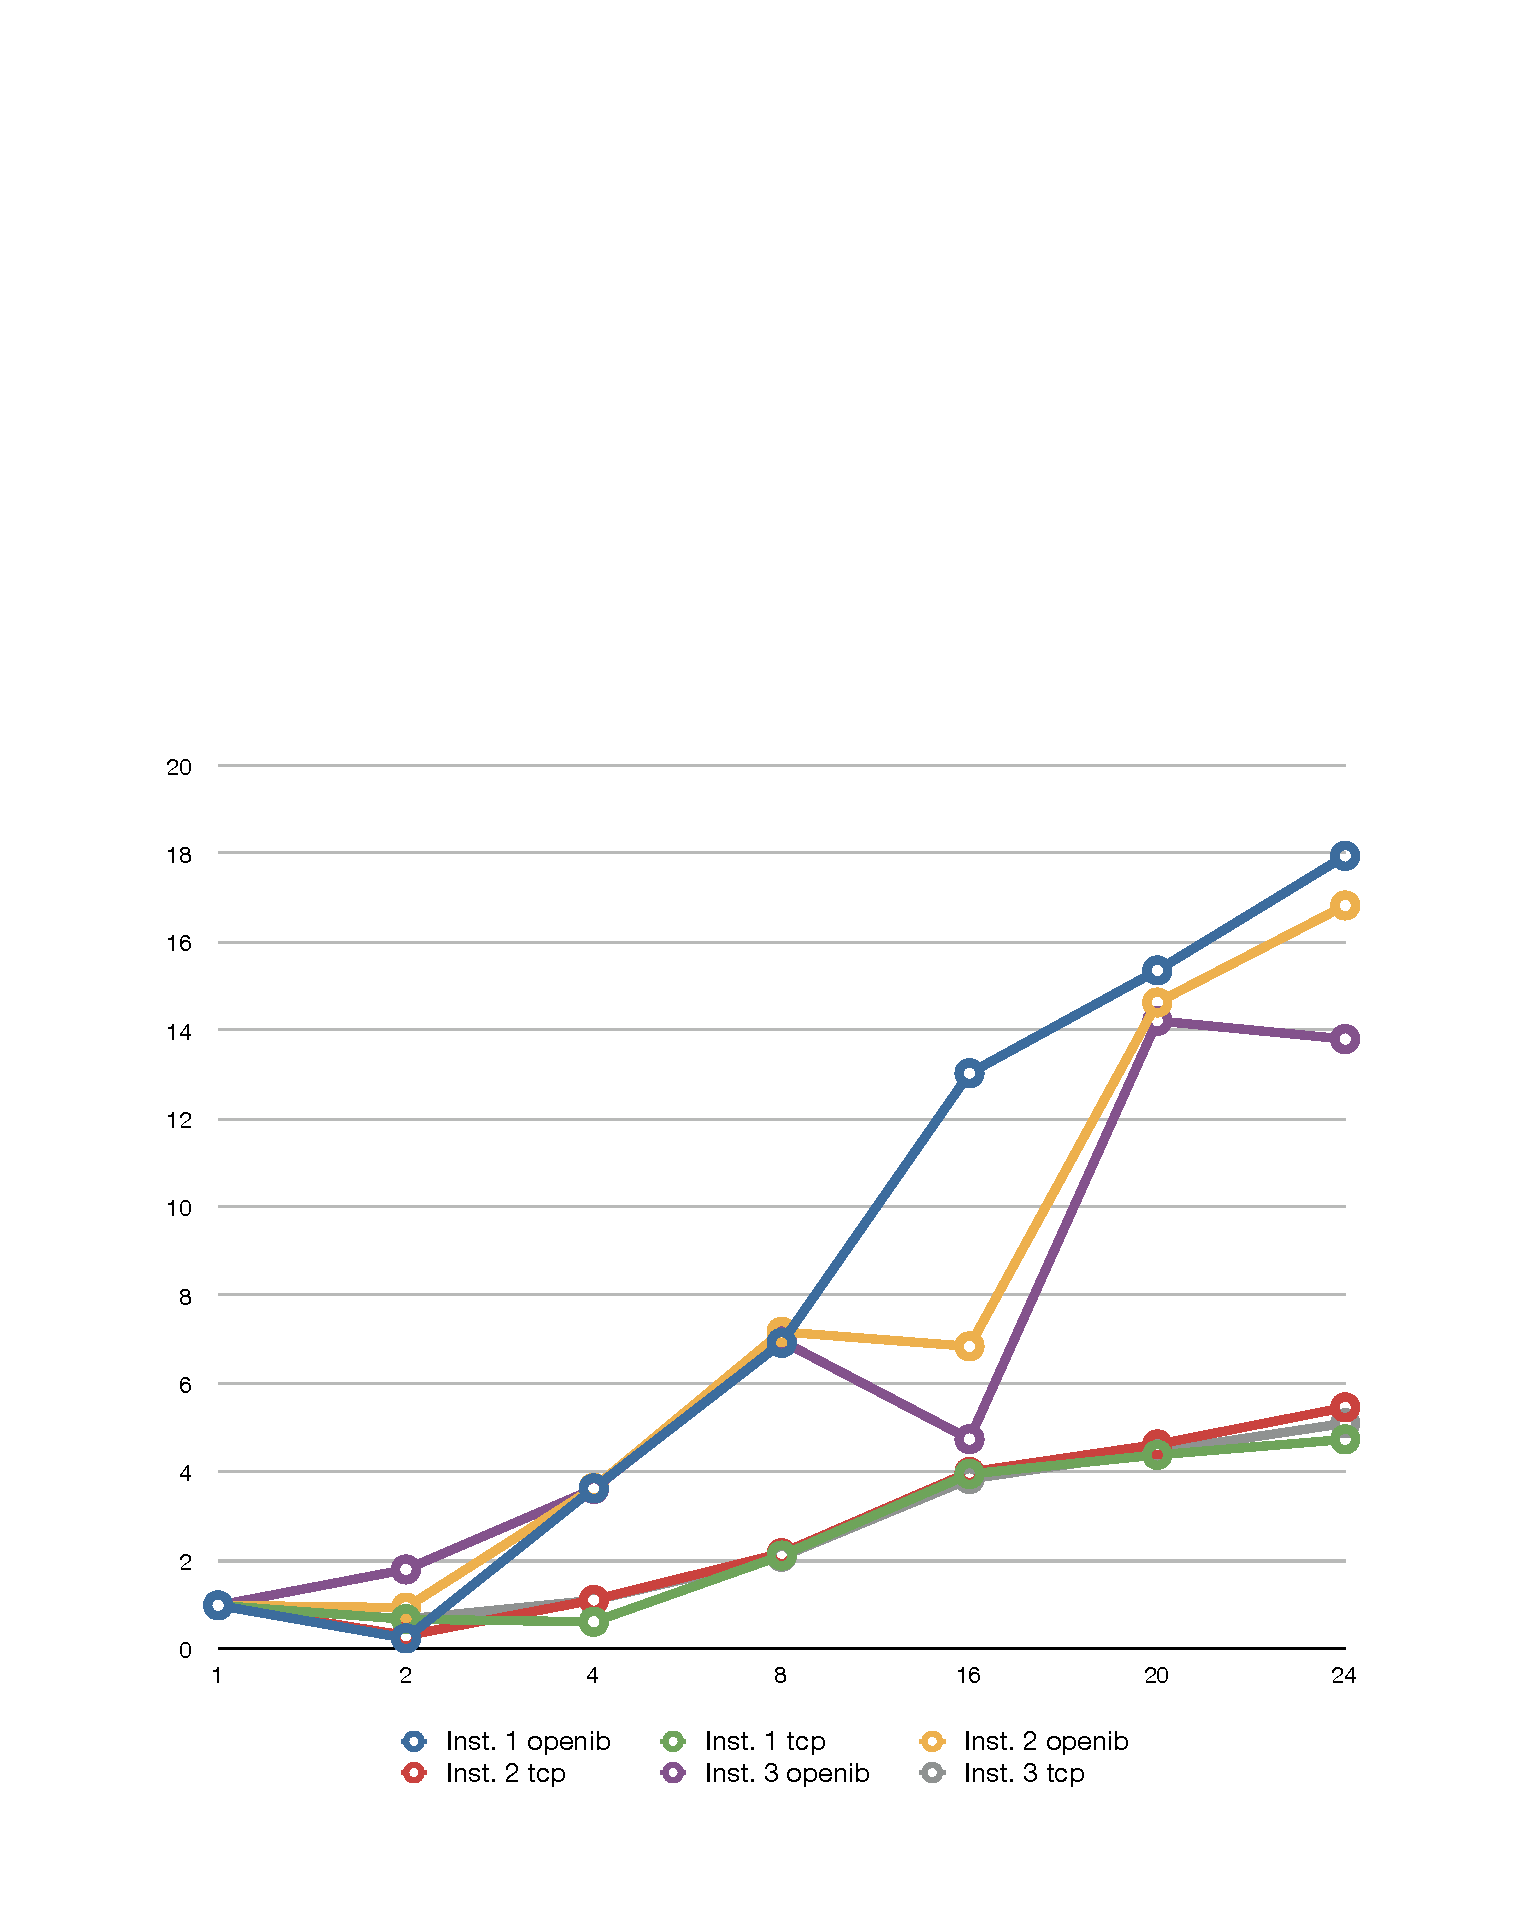
\includegraphics[width=\textwidth]{graph.pdf}}
\caption{Graf relativniho zrychleni vypoctu}
\label{graph}
\end{figure}

\subsection{Vyhodnoceni}
K superlinearnimu zrychleni nedoslo. Vysledky ukazuji, ze paralelni algoritmus byl vyhotoven
kvalitne, v nejlepsim pripade je zpomaleni komunikaci mezi procesory a rozdelovanim prace
jen 25\%. Mereni take ukazalo, ze sit Ethernet je v prumeru o 45\% pomalejsi, nez
sit InfiniBand.

\begin{figure}[ht]
\centerline{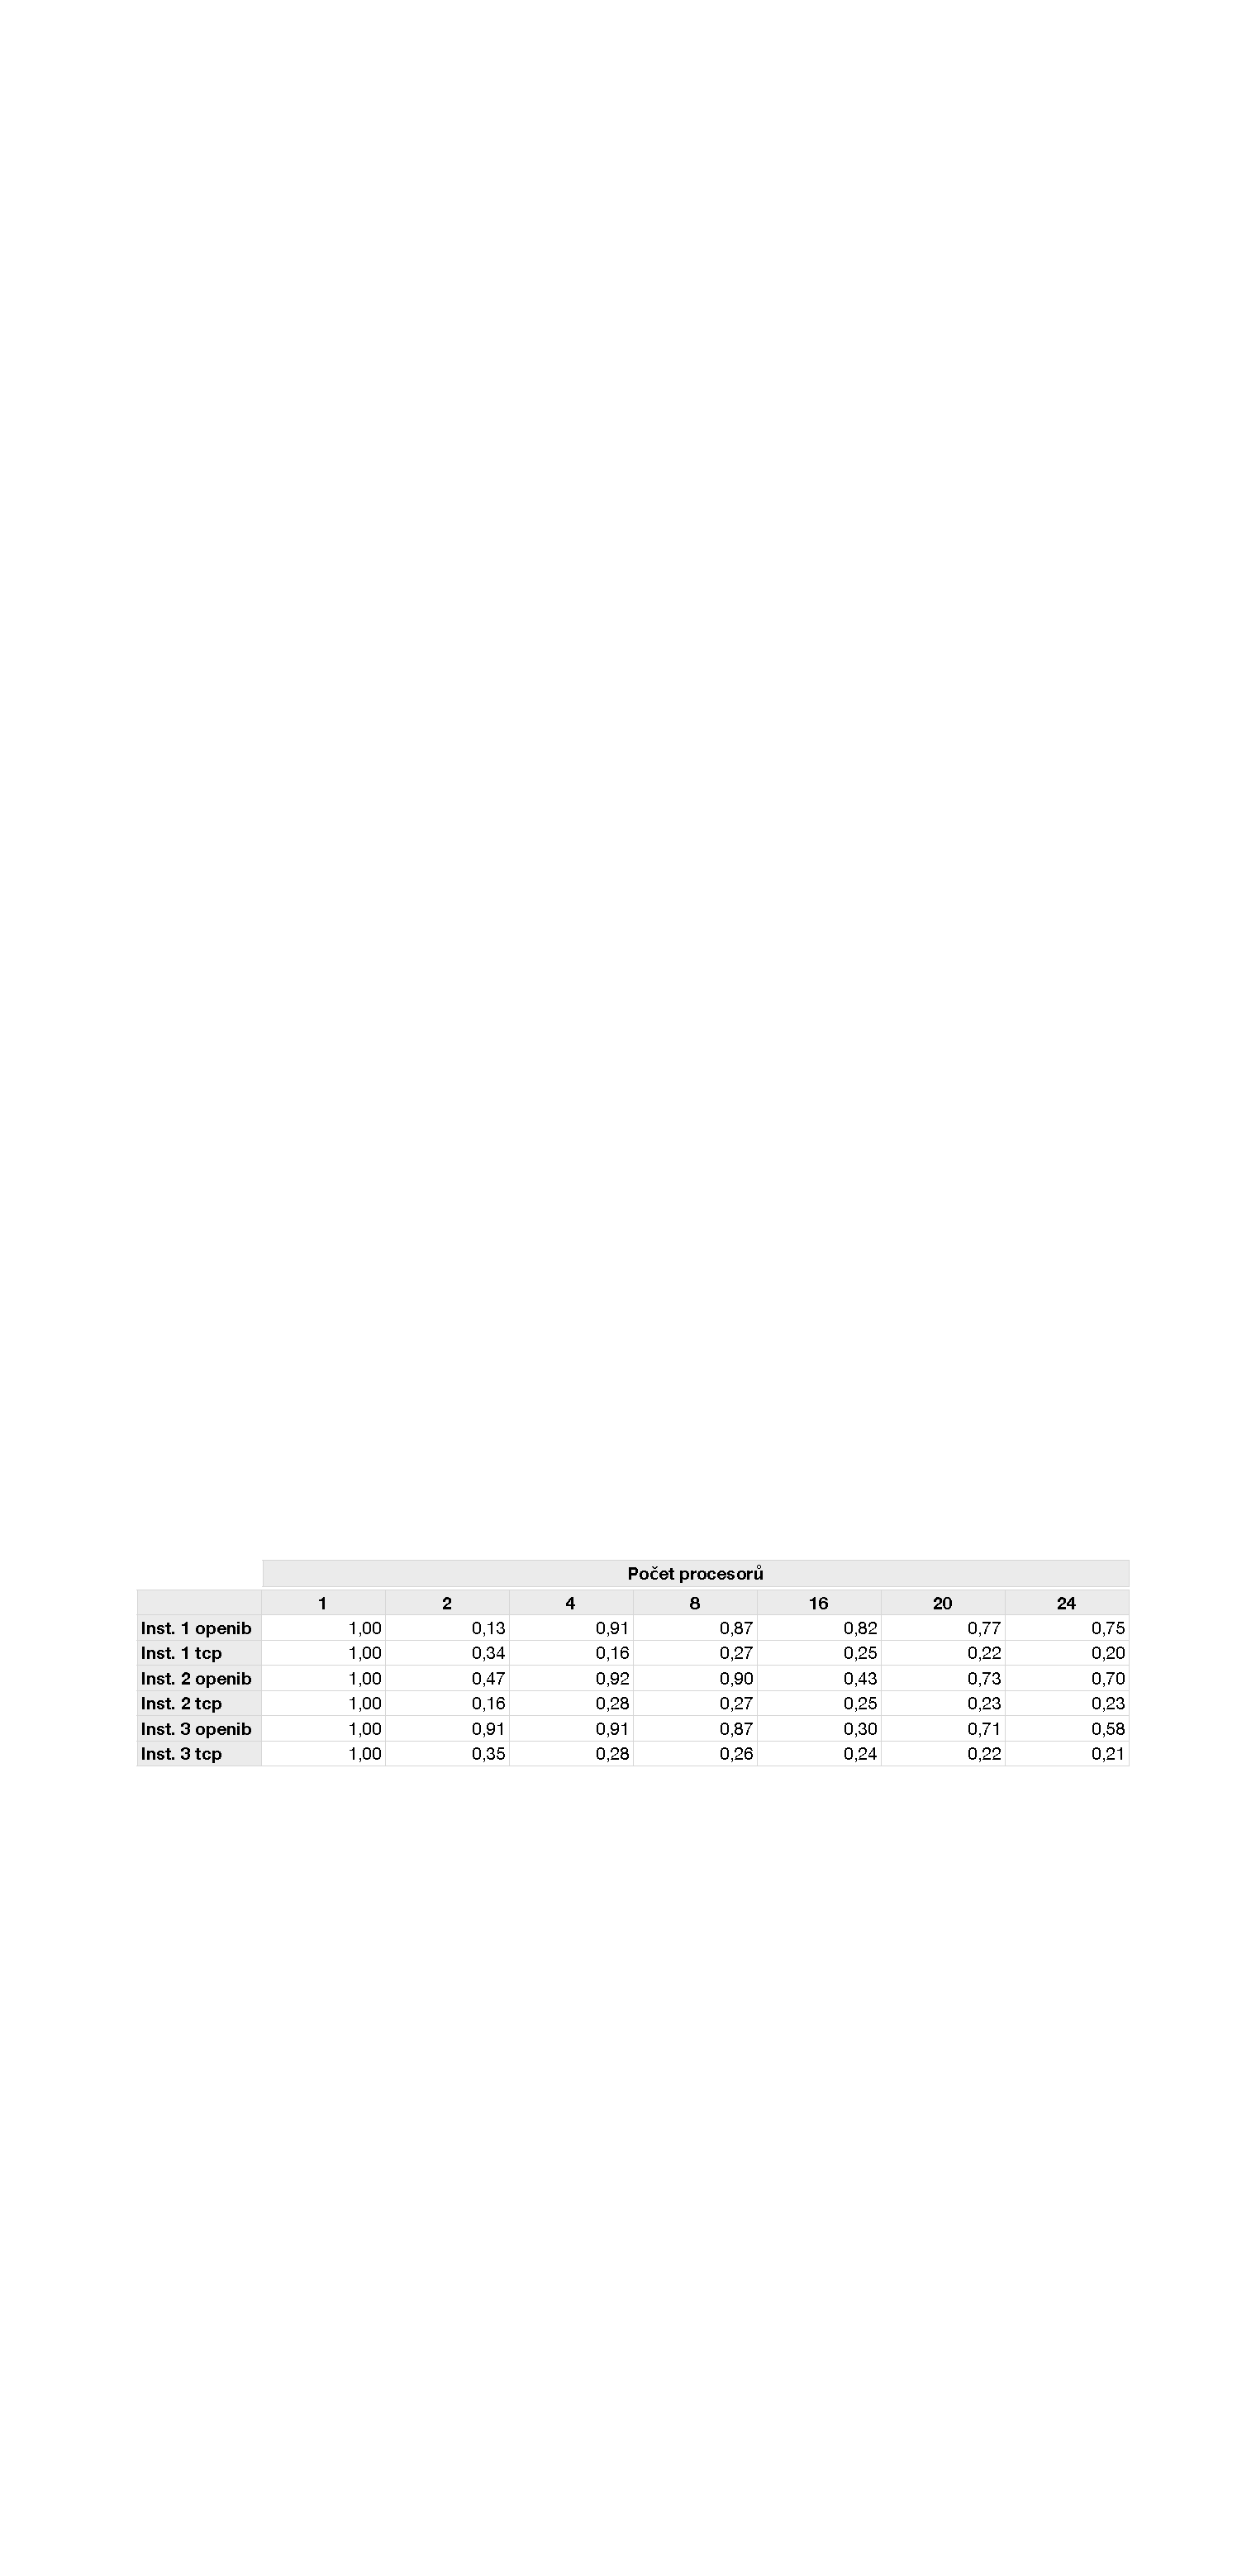
\includegraphics[width=\textwidth]{table-rel-per-cpu.pdf}}
\caption{Relativni zrychleni vypoctu proti sekvencnimu algoritmu na pocet porcesoru}
\label{table-rel-per-cpu}
\end{figure}

\begin{figure}[ht]
\centerline{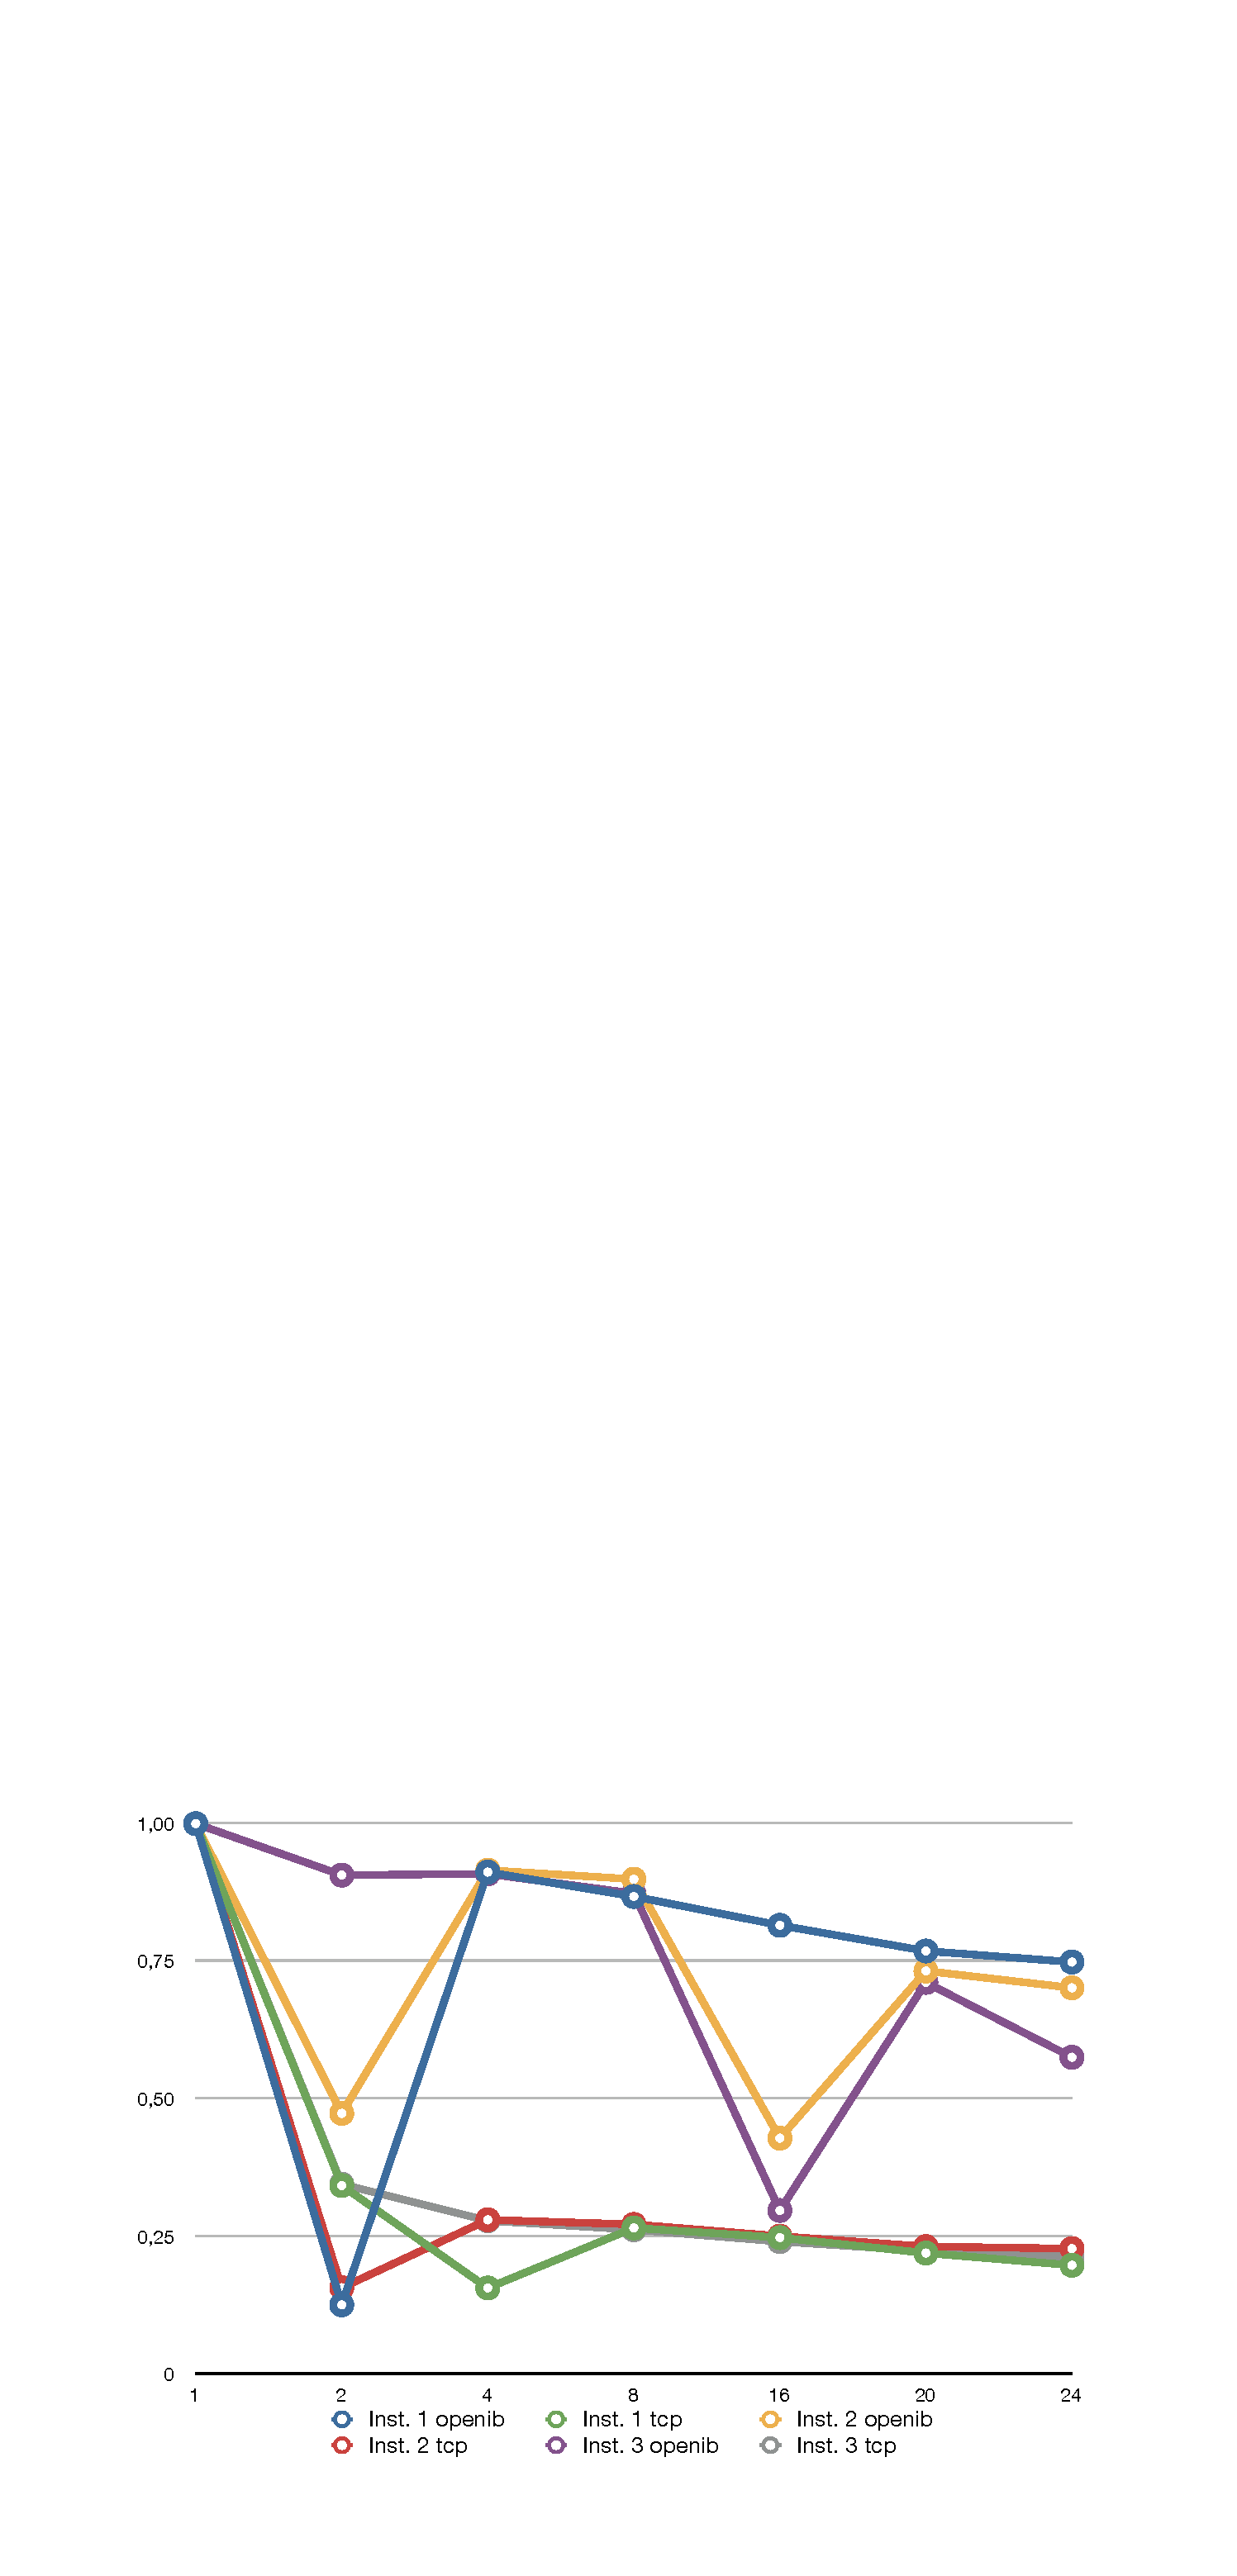
\includegraphics[width=\textwidth]{graph-per-cpu.pdf}}
\caption{Graf relativniho zrychleni vypoctu na pocet porcesoru}
\label{graph-per-cpu}
\end{figure}

\section{Literatura}

\begin{itemize}
	\item Podklady na starankach predmetu (https://service.felk.cvut.cz/courses/X36PAR/)
\end{itemize}

\end{document}








